%%%%%%%%%%%%%%%%%%%%%%%%%%%%%%%%%%%%%%%%%%%%%%%%%%%%%%%%%%%%%%%%%%%%%%%%%%%%%%%
% Rownanie na faze
%%%%%%%%%%%%%%%%%%%%%%%%%%%%%%%%%%%%%%%%%%%%%%%%%%%%%%%%%%%%%%%%%%%%%%%%%%%%%%%
\subsection{Czwórka symetryczna kierunków zerowych.}
Od tego momentu zakładamy, że wersor $e_3$ jest prostopadły do 
hiperpłaszczyzny ruchu tak, że
$A\cdot e_3 = 0$.
%Zawsze możemy wybrać bazę $E$ tak, aby powyższy warunek był 
%spełniony~(zob. dodatek~\ref{e3proof}). 
Nie jest to zbyt restrykcyjne założenie i pozwala 
na zastosowanie modelu w wielu przypadkach.
Zauważmy, że wtedy wektor~$A$~leży w płaszczyźnie rozpinanej przez 
wektory~$e_1$~i~$e_2$. Liczymy przyspieszenie właściwe~$\alpha$ i 
dostajemy
\begin{align*}
\alpha^2 = (A\cdot e_1)^2 + (A\cdot e_2)^2.
\end{align*}
Interpretując poprzednią równość jako trójkę pitagorejską 
możemy wprowadzić następujące oznaczenia
\begin{align*}
\cos\chi = \frac{A\cdot e_1}{\alpha},\\
\sin\chi = \frac{A\cdot e_2}{\alpha}.
\end{align*}

Z wersorów $e$ i $e_3$ tworzymy dwa zerowe wektory $k_+$ i $k_-$
skierowane w przyszłość, 
które uważamy za wektory własne pewnej transformacji Lorentza. 
\begin{align}
k_+ &= \frac{e+e_3}{\sqrt{2}} ,\\
k_- &= \frac{e-e_3}{\sqrt{2}} ,
\end{align}
\begin{align*}
k_+\cdot k_- = 1, \qquad k_\pm\cdot k_\pm  = 0.
\end{align*}
Wektory te są wektorami własnymi pewnego obrotu $\mathcal{O}$.
\begin{align*}
\mathcal{O}( k_\pm ) = \frac{1}{\sqrt{2}} \mathcal{O} 
(e\pm e_3) =\frac{1}{\sqrt{2}} 
(\mathcal{O} e\pm \mathcal{O} e_3) =
\frac{1}{\sqrt{2}}  (e\pm e_3) = k_\pm.
\end{align*}
 Łatwo sprawdzić, że 
jest 
to obrót w płaszczyźnie wyznaczonej przez wersory~$e_1$ i $e_2$,
czyli eliptyczne przekształcenie \begin{wrapfigure}[15]{r}{5cm}
\centering
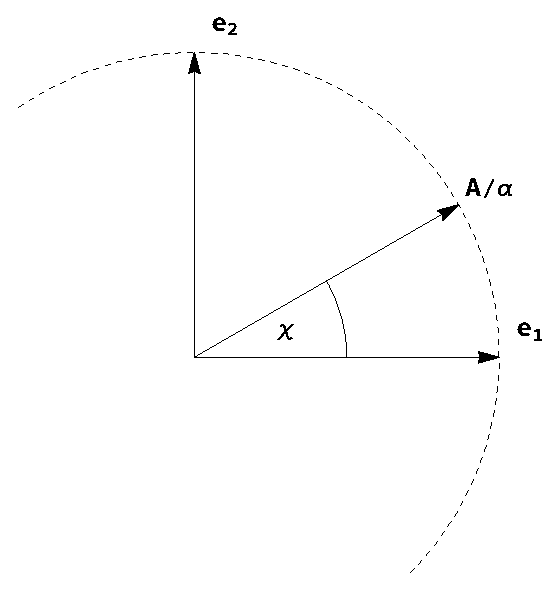
\includegraphics[scale=0.5]{A_chi.eps}
\caption{Schemat obrazujący obrót~$\mathcal{O}$ wykonany na wersorze 
przyspieszenia $A/\alpha$ w bazie $E$.}{\label{A_chi_plot}}
\end{wrapfigure}Lorentza. 
Obrót ten pozwala nam zinterpretować kąt~$\chi$. 
Zauważmy, że możemy za pomocą obrotu~$\mathcal{O}$ obrócić, 
wersor wektora przyspieszenia~o kąt~$-\chi$ 
tak, aby spełniał prawo transportu~\eqref{FW}. 
Schematycznie przedstawiono to na rysunku~\ref{A_chi_plot}.

Rozważamy trzeci wektor zerowy $k$ skierowany w przyszłość taki, 
że $k\cdot e_3 \equiv 0$ oraz $k(0)\cdot e_1(0) =0$.  
%Z pierwszego warunku wynika że ostatnia współrzędna wektora $k$ 
%jest zerowa. $e_1(0)=(0,1,0,0)$ co oznacza, że 
%wektor $k(0)$ ma drugą współrzędną równą zero. 
Wektor $k$ rozkładamy w bazie $E$
\begin{align*}
k = k^0 e +  k^i e_i, \qquad k^1(0)=0, k^3 = 0,
\end{align*}
\begin{align*}
k(0) = k^0(0) e(0) + k^2(0) e_2(0) .
\end{align*}
Rozkładając $k$ w bazie $E$ stwierdzamy, że jego współrzędne 
formują trójkę pitagorejską 
\begin{align}
(k \cdot e)^2 = (k \cdot e_1)^2 +  (k \cdot e_2)^2 .
\end{align}
\\
Kierunek zerowy $k$ odpowiada kierunkowi wskazówki zegara. 
 W przypadku, gdy byłyby 
dwie wskazówki poruszające się po tym samym okręgu ale w 
przeciwnych kierunkach moglibyśmy kolejne tyknięcia zegara
wyznaczyć przez punkty spotkania się wskazówek. 
Jednak nasz zegar wyposażony jest w jedną wskazówkę i 
potrzebujemy kierunku odniesienia, względem którego będziemy 
mierzyć jego wskazania. Fazę zegara definiujemy względem reperu
przenoszonego transportem~\eqref{FW}, gdyż taki reper nie 
rotuje względem obserwatora, co umożliwia mierzenie  
fazy zegara względem wersorów bazy. 
Wprowadzamy \textbf{fazę zegara} $\varphi$ 
równością
\begin{align}\label{phi_definition}
\cos\varphi = \frac{k\cdot e_1}{k\cdot e} ,
\end{align}
\begin{align*}
k = (k\cdot e) (e -\cos\varphi e_1 - \sin\varphi e_2 ).
\end{align*}
%gdzie $k^0=k\cdot e$, $k^1=-k\cdot e_1$, $k^2=-k\cdot e_2$.
Z wektora $k(0)$ tworzymy wektor zerowy $k_0(s)$ tak, aby spełniał 
prawo transportu~\eqref{FW}. Będzie on kierunkiem odniesienia 
w zegarze. Wiemy, że wtedy jego współrzędne~w 
bazie~$E$ są stałe. Niech zatem
$k_0(s) =  \sqrt{2} (e + e_2)$.
Warunek początkowy na fazę $\varphi$ ustalamy jako
$\varphi(0)=-\frac{\pi}{2}$. Wtedy dla $s=0$ wektory
$k$ i $k_0$ reprezentują ten sam kierunek zerowy. 
%Z warunku uzyskujemy równość 
%\begin{align*}
%\frac{\d k_0(s)\cdot e }{\d s} = 0.
%\end{align*}
%Rozpiszemy drugi warunek
%\begin{align*}
%k_0(s)_\perp = -(k_0(s)\cdot e_2)e_2
%\end{align*}
%\begin{align*}
%\frac{\d -(k_0(s)\cdot e_2)e_2 }{\d s}
% =-\frac{\d (k_0(s)\cdot e_2)}{\d s}e_2 - (k_0(s)\cdot e_2)\dot{e_2} 
%\end{align*}
%\begin{align*}
%\left( \frac{\d -(k_0(s)\cdot e_2)e_2 }{\d s}\right)_\perp =
%-\frac{\d (k_0(s)\cdot e_2)}{\d s}\left(e_2 \right)_\perp 
%-(k_0(s)\cdot e_2)\left(\dot{e_2} \right)_\perp 
%\end{align*}
%Z konstrukcji bazy mamy
%\begin{align*}
%\left(\dot{e_2} \right)_\perp  = 0, \qquad \left(e_2 \right)_\perp  = e_2
%\end{align*}
%co daje zerowanie równość
%\begin{align*}
%\frac{\d k_0(s)\cdot e_2 }{\d s} = 0.
%\end{align*}
%Z powyższych warunków widzimy, że współrzędne wektora 
%$k_0(0)$ w bazie $Z$ muszą być stałe. 
%Uwzględniając, że wektor ma być zerowy wybieramy następujący wektor
%\begin{align}
%k_0(s) = e + e_2 =  (1,0,1,0)_Z \tag{k0} \label{eq:k0}
%\end{align}
Każdemu kierunkowi zerowemu możemy przyporządkować punkt na sferze,
a następnie każdemu punktowi sfery możemy przyporządkować,
przez rzut stereograficzny, 
punkt z płaszczyzny zespolonej 
(odpowiednio uzwarconej)~\cite{star1993algebra}.
Mówimy, że wektory zerowe tworzą czwórkę symetryczną,
 kiedy dwustosunek odpowiadających im liczb zespolonych 
 wynosi $e^{\pm i\pi/3}$.  
Dwustosunek liczb zespolonych $z_0,\ z_1,\ z_2,\ z_3$ przyjmujemy w 
postaci wyrażonej równością~\eqref{dwustosunek_definicja}~\cite{star1993algebra}.
Skonstruujemy teraz czwarty wektor zerowy $k_3$, który razem z 
wektorami $k_+$, $k_0$, $k_-$ utworzy czwórkę symetryczną.
Liczby zespolone odpowiadające wektorom własnym $k_\nu$ oznaczamy
przez $\kappa_\nu$, gdzie $\nu \in \{+,\ 0,\ -,\ 3\}$.
W zależności od kolejności wektorów i 
przyjętego znaku w wykładniku eksponenty~\eqref{dwustosunek_kappa}
otrzymujemy dwie liczby $\kappa_3$ różniące się znakiem części 
rzeczywistej \eqref{kappa3_wynikPM}. 
\begin{align}\label{dwustosunek_definicja}
(z_0z_1z_2z_3) = 
\frac{(z_0-z_1)}{(z_0-z_3)} 
\frac{(z_2-z_3)}{(z_2 -z_1)} .
\end{align}
\begin{align}\label{dwustosunek_kappa}
\kappa_0 = i,\ \kappa_+ = 0,\ \kappa_-=\infty,
\qquad (\kappa_0\kappa_+\kappa_-\kappa_3),
 = e^{\pm i\pi/3} \\ \label{kappa3_wynikPM}
\kappa_3 =\pm  \frac{\sqrt{3}}{2} + \frac{i}{2}, \qquad
k_3 = \sqrt{2} e\pm \frac{\sqrt{3}}{\sqrt{2}}e_1+ \frac{1}{\sqrt{2}} e_2 ,
\end{align}
\begin{align*}
k_\mu \cdot k_\nu = 1 , 
\quad k_\nu \cdot k_\nu = 0,\quad \mu \neq \nu ,\ 
\mu,\ \nu \in \{0,\ +,\ -,\ 3\}.
\end{align*} 
Niech teraz wektorowi zerowemu~$k$ odpowiada 
liczba $\kappa_\varphi$~\eqref{kappa}.
Na rysunkach~4a i 4b
widzimy wzajemne położenie 
uzyskanej czwórki symetrycznej (dla Re$ (\kappa_3) >0$) 
oraz obrazu wektora $k$. 
Uzyskane wektory są liniowo niezależne i tworzą bazę 
kierunków zerowych, która dodatkowo spełnia 
prawo transportu~\eqref{FW}.
\begin{align}\label{kappa}
\kappa_\varphi = -\cos\varphi - i \sin \varphi .
\end{align}
\begin{figure}[h]
\begin{minipage}[b]{.5\linewidth}
\centering
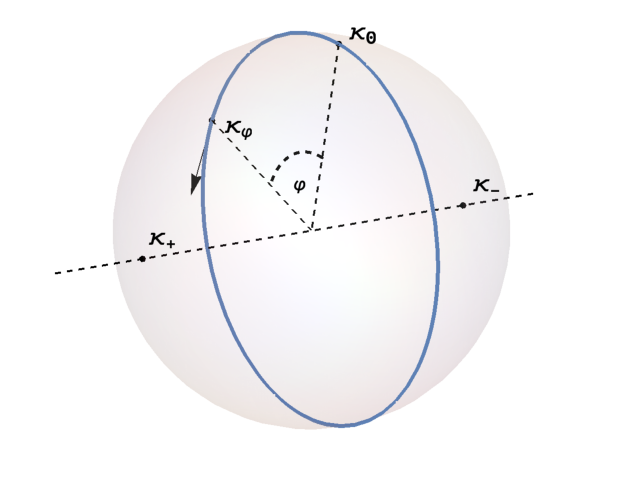
\includegraphics[scale=0.62]{dwustosunek_sfera.eps}
\subcaption{}
\end{minipage}%
\begin{minipage}[b]{.5\linewidth}
\centering
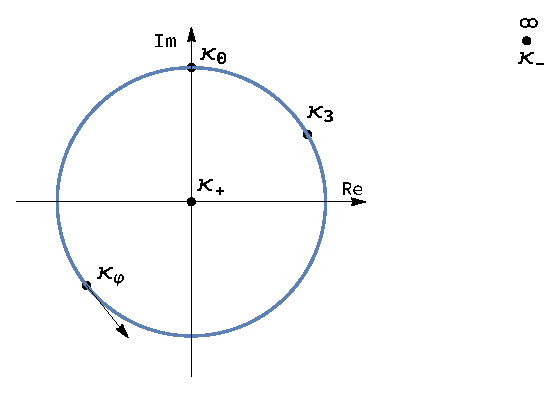
\includegraphics[scale=0.8]{dwustosunek_plaszczyzna.eps}
\subcaption{}
\end{minipage}
\caption{Obraz czwórki symetrycznej oraz kierunku $k$ na płaszczyźnie 
zespolonej~(a) oraz na sferze jednostkowej~(b).
Punkt $\kappa_\varphi$ porusza się po zaznaczonym okręgu jednostkowym 
wraz ze wzrostem $\varphi$. Wektorem stycznym do okręgu zaznaczono 
kierunek ruchu.}
\label{dwustosunek_plaszczyzna}
\end{figure}
\\

